%! Author = Ian's PC
%! Date = 9/11/2023

% Preamble
\documentclass[11pt]{article}

% Packages
\usepackage{amsmath}
\usepackage{romannum}
\usepackage{graphicx}

% Document
\begin{document}
    Assignment 1 of CS376. Ian Chen, ic8683\newline
    
    \textbf{Part \Romannum{1}.}\newline

    \textbf{1. What are the three applications of image filtering?}\newline
    Edge detection, template matching, texture analysis and synthesis.\newline

    \textbf{2. What is the difference between the mean filtering and the median filtering?}\newline
    Median filtering is non-linear and preserves edges while mean smoothes out the image.
    Median retains all existing pixel values and doesn’t create new values. Median also removes spikes and salt \& pepper noise.\newline

    \textbf{3. In class, we talked about image smoothing followed by computing image gradients.
    Is it identical to computing image gradients first and then perform image smoothing on the resulting image gradients?}\newline
    No, it’s different, since the paths will likely change if blurring$\rightarrow$calculate seam vs. calculate seam$\rightarrow$blurring.\newline
    
    \textbf{4. How to take the advantage of the separability of a filter for fast image filtering calculation?}\newline
    We can convolve the rows and columns of the image separately, each using its own matrix operation. This makes the image filtering more efficient.\newline

    \textbf{5. In non-maximum suppressing, we detect the maximum pixel along the image gradient direction. Provide examples where this approach is sub-optimal.
    You can draw illustrations or provide results on real examples. Please provide a short justification (2-3 sentences) on why this is the case.}\newline
    
    \textbf{Extra credit (5points). So far we have covered filtering and edge detection for images. Please mention how to extend the idea to videos.
    Please discuss how to de-noise in both the spatial and/or temporal domain, how to compute gradients in the spatial and/or temporal domain,
        and how to detect ”edges” in the spatial and/or temporal domain.}\newline

    \textbf{Part \Romannum{2}.}\newline
    
    \textbf{Question 1:}\newline
    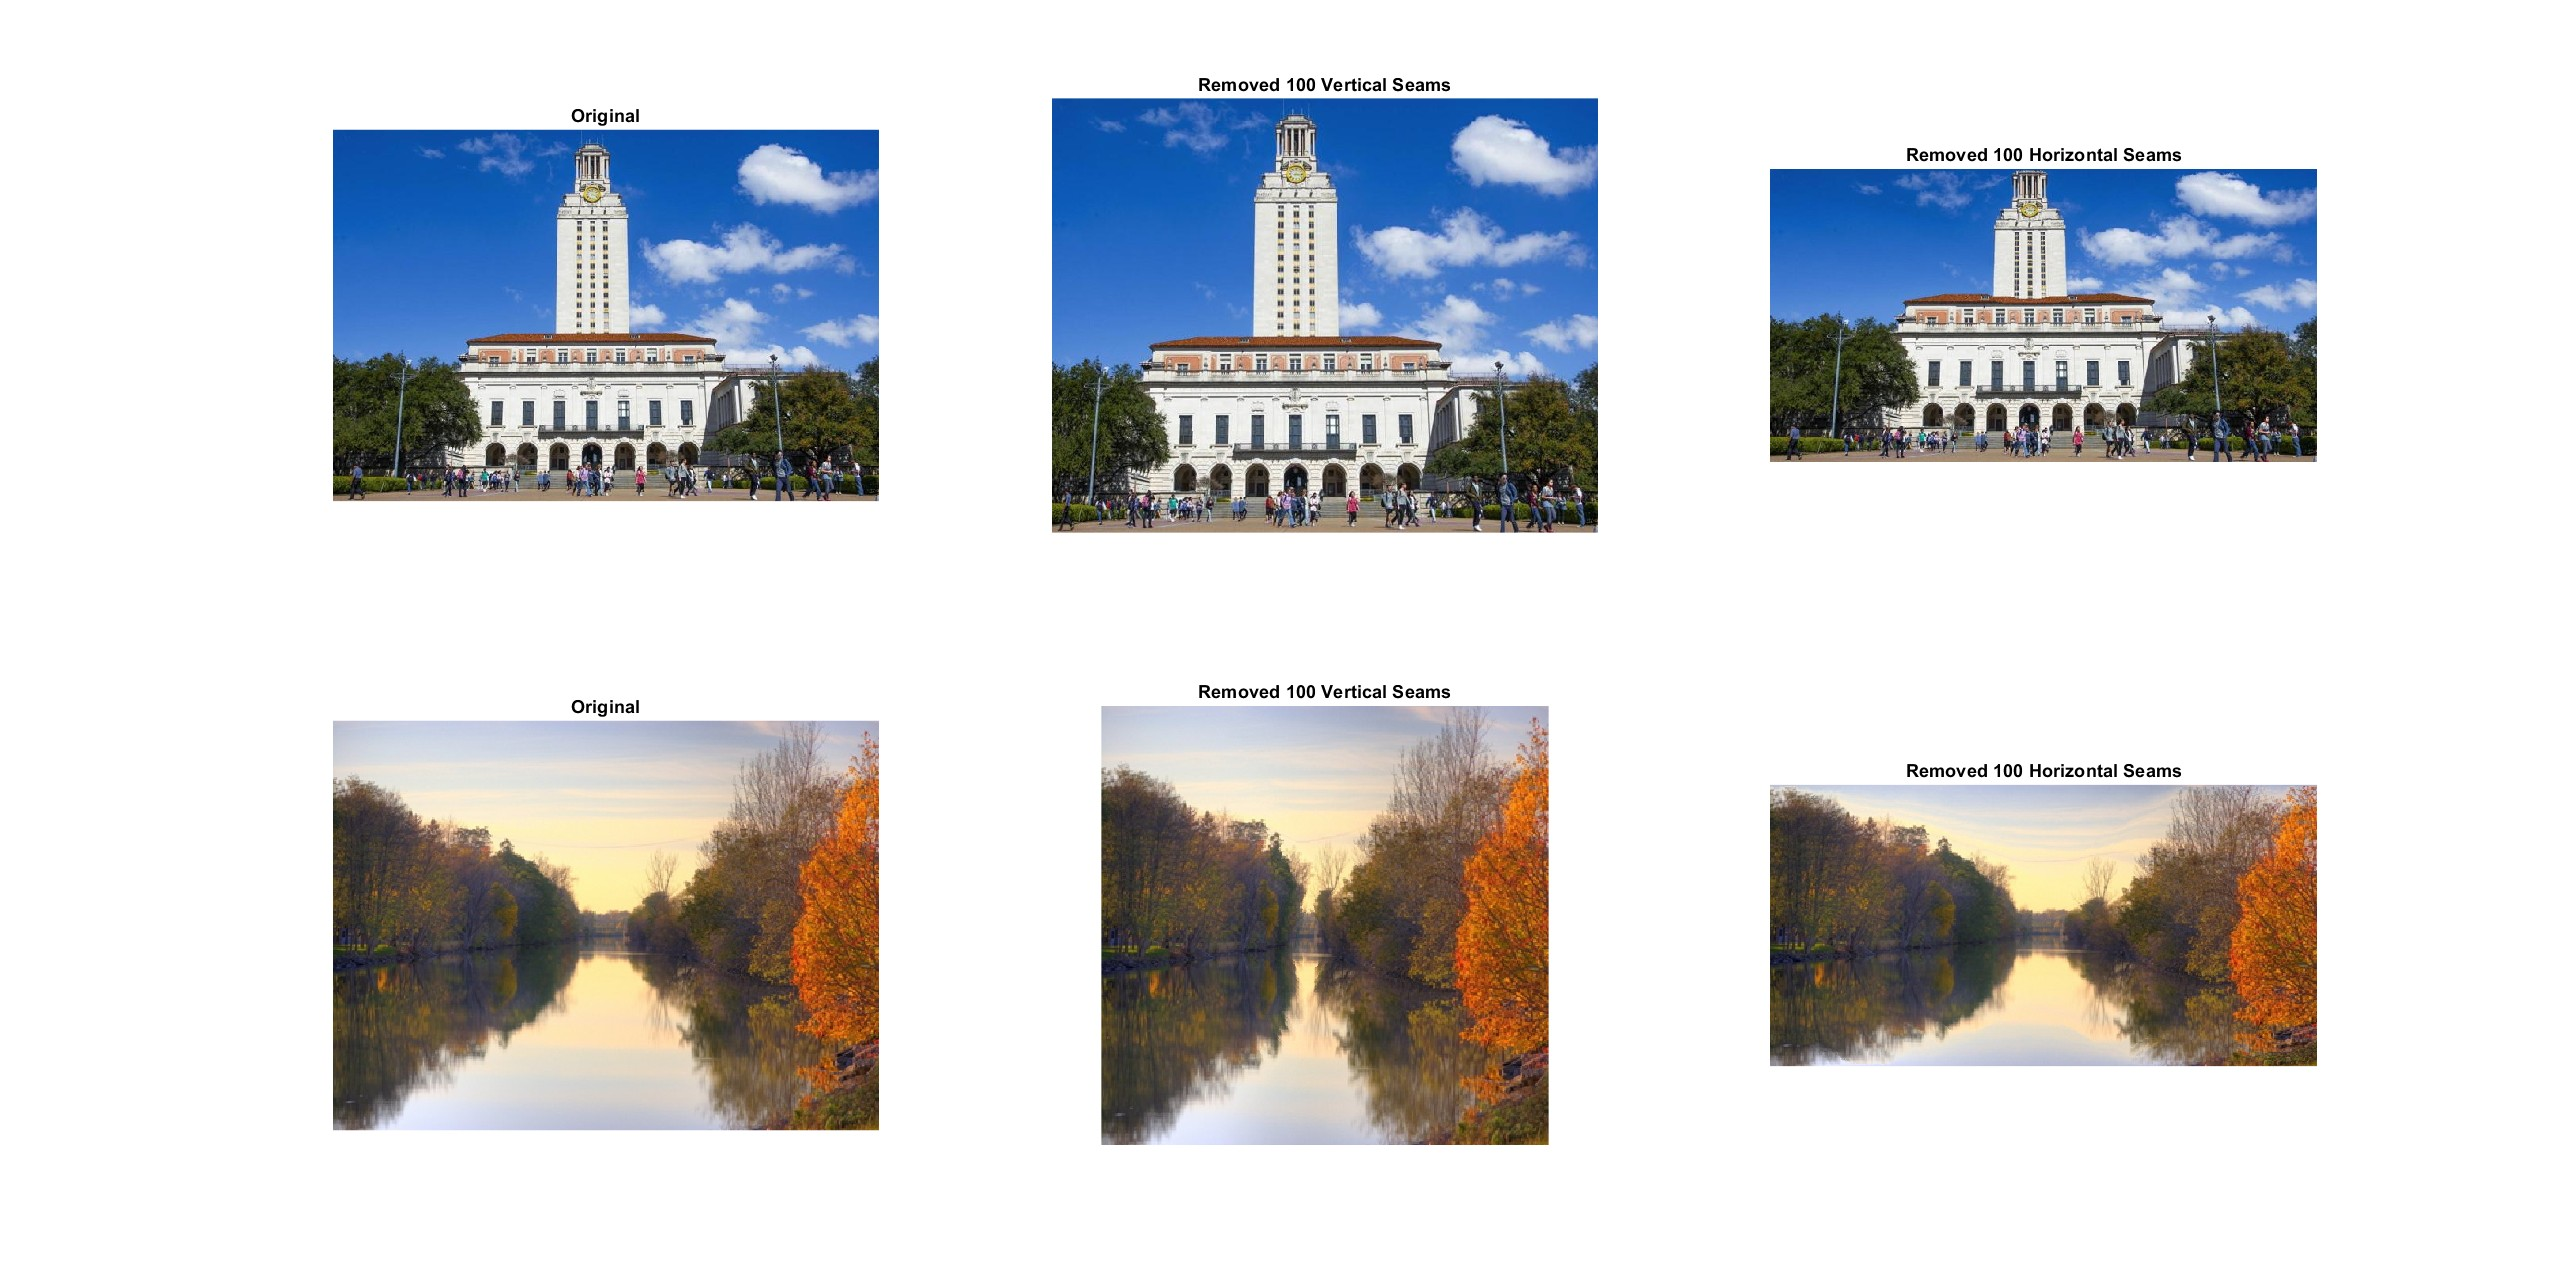
\includegraphics[width=\linewidth]{Part 2 Pictures/question1}\newline

    \textbf{Question 2:}\newline
    The reason for these outputs is that on top of each object there's a
    triangle pointing to it, since for a object or background, the gradient
    is small, but, when edges to objects are detected through large
    gradients, the energy path will prioritize other paths which don't pass
    through many edges.\newline
    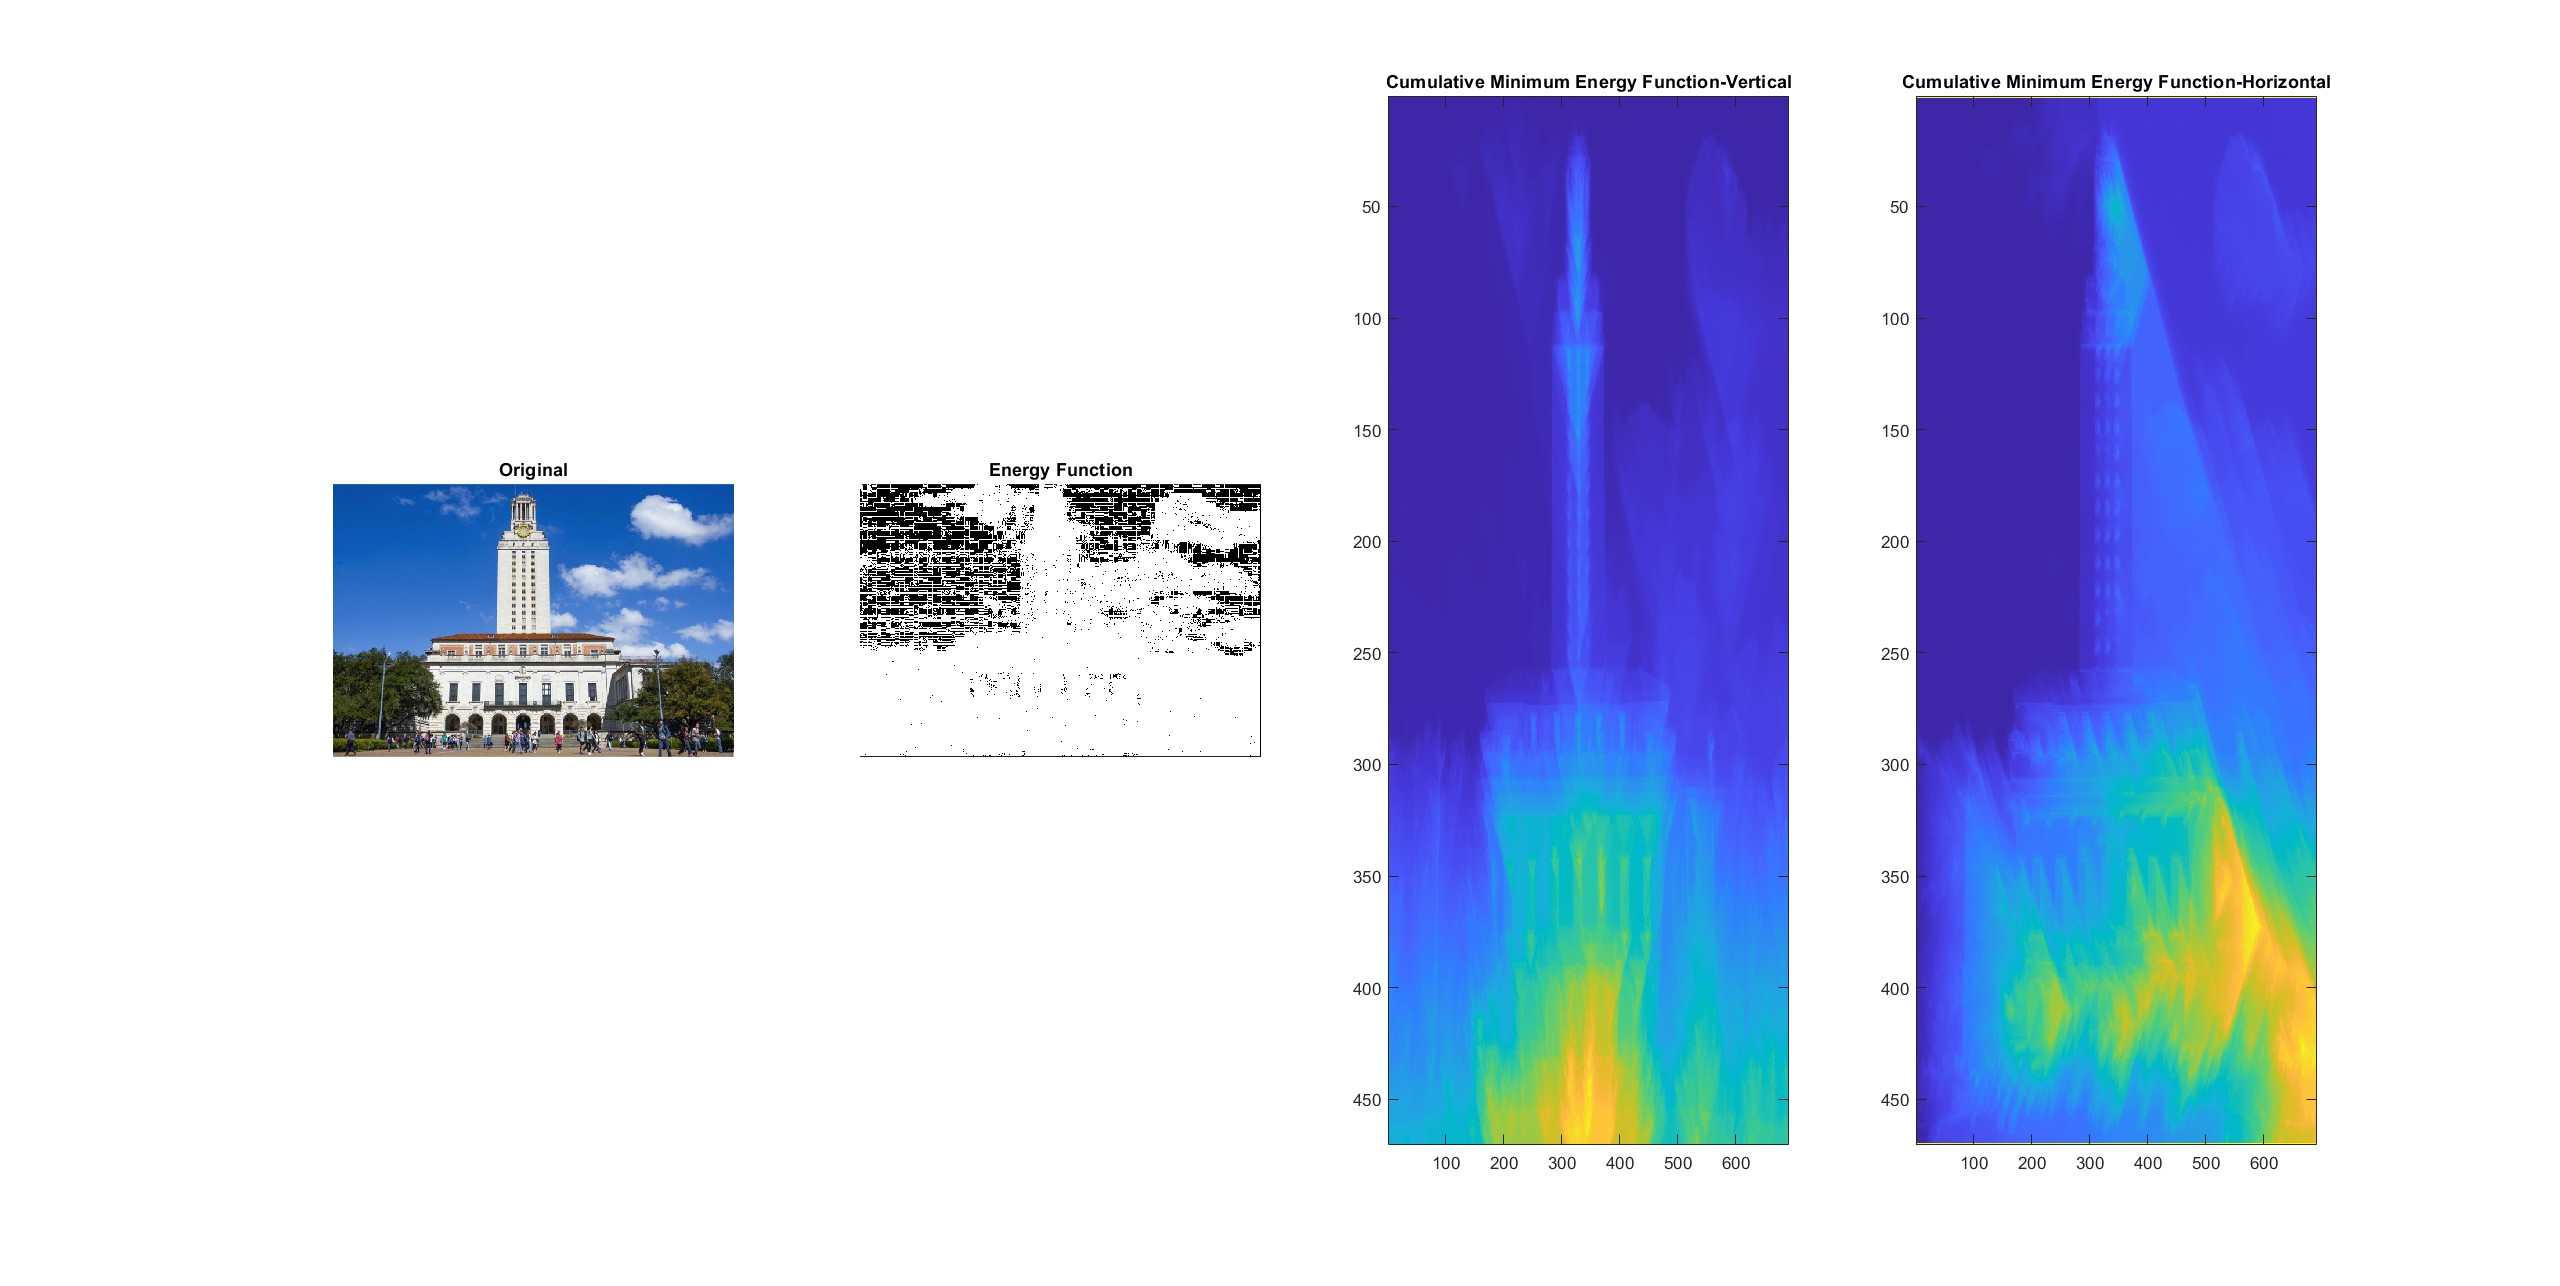
\includegraphics[width=\linewidth]{Part 2 Pictures/question2}\newline

    \textbf{Question 3:}\newline
    These are the optimal seams since they include the blue sky background,
    which is mostly the same color. Therefore, their cumulative gradient will
    be small. However, in the vertical gradient, the trees in the foreground
    cover the entire bottom half, so the path passed through the patch which
    are mostly the same shade of the tree leaves.\newline
    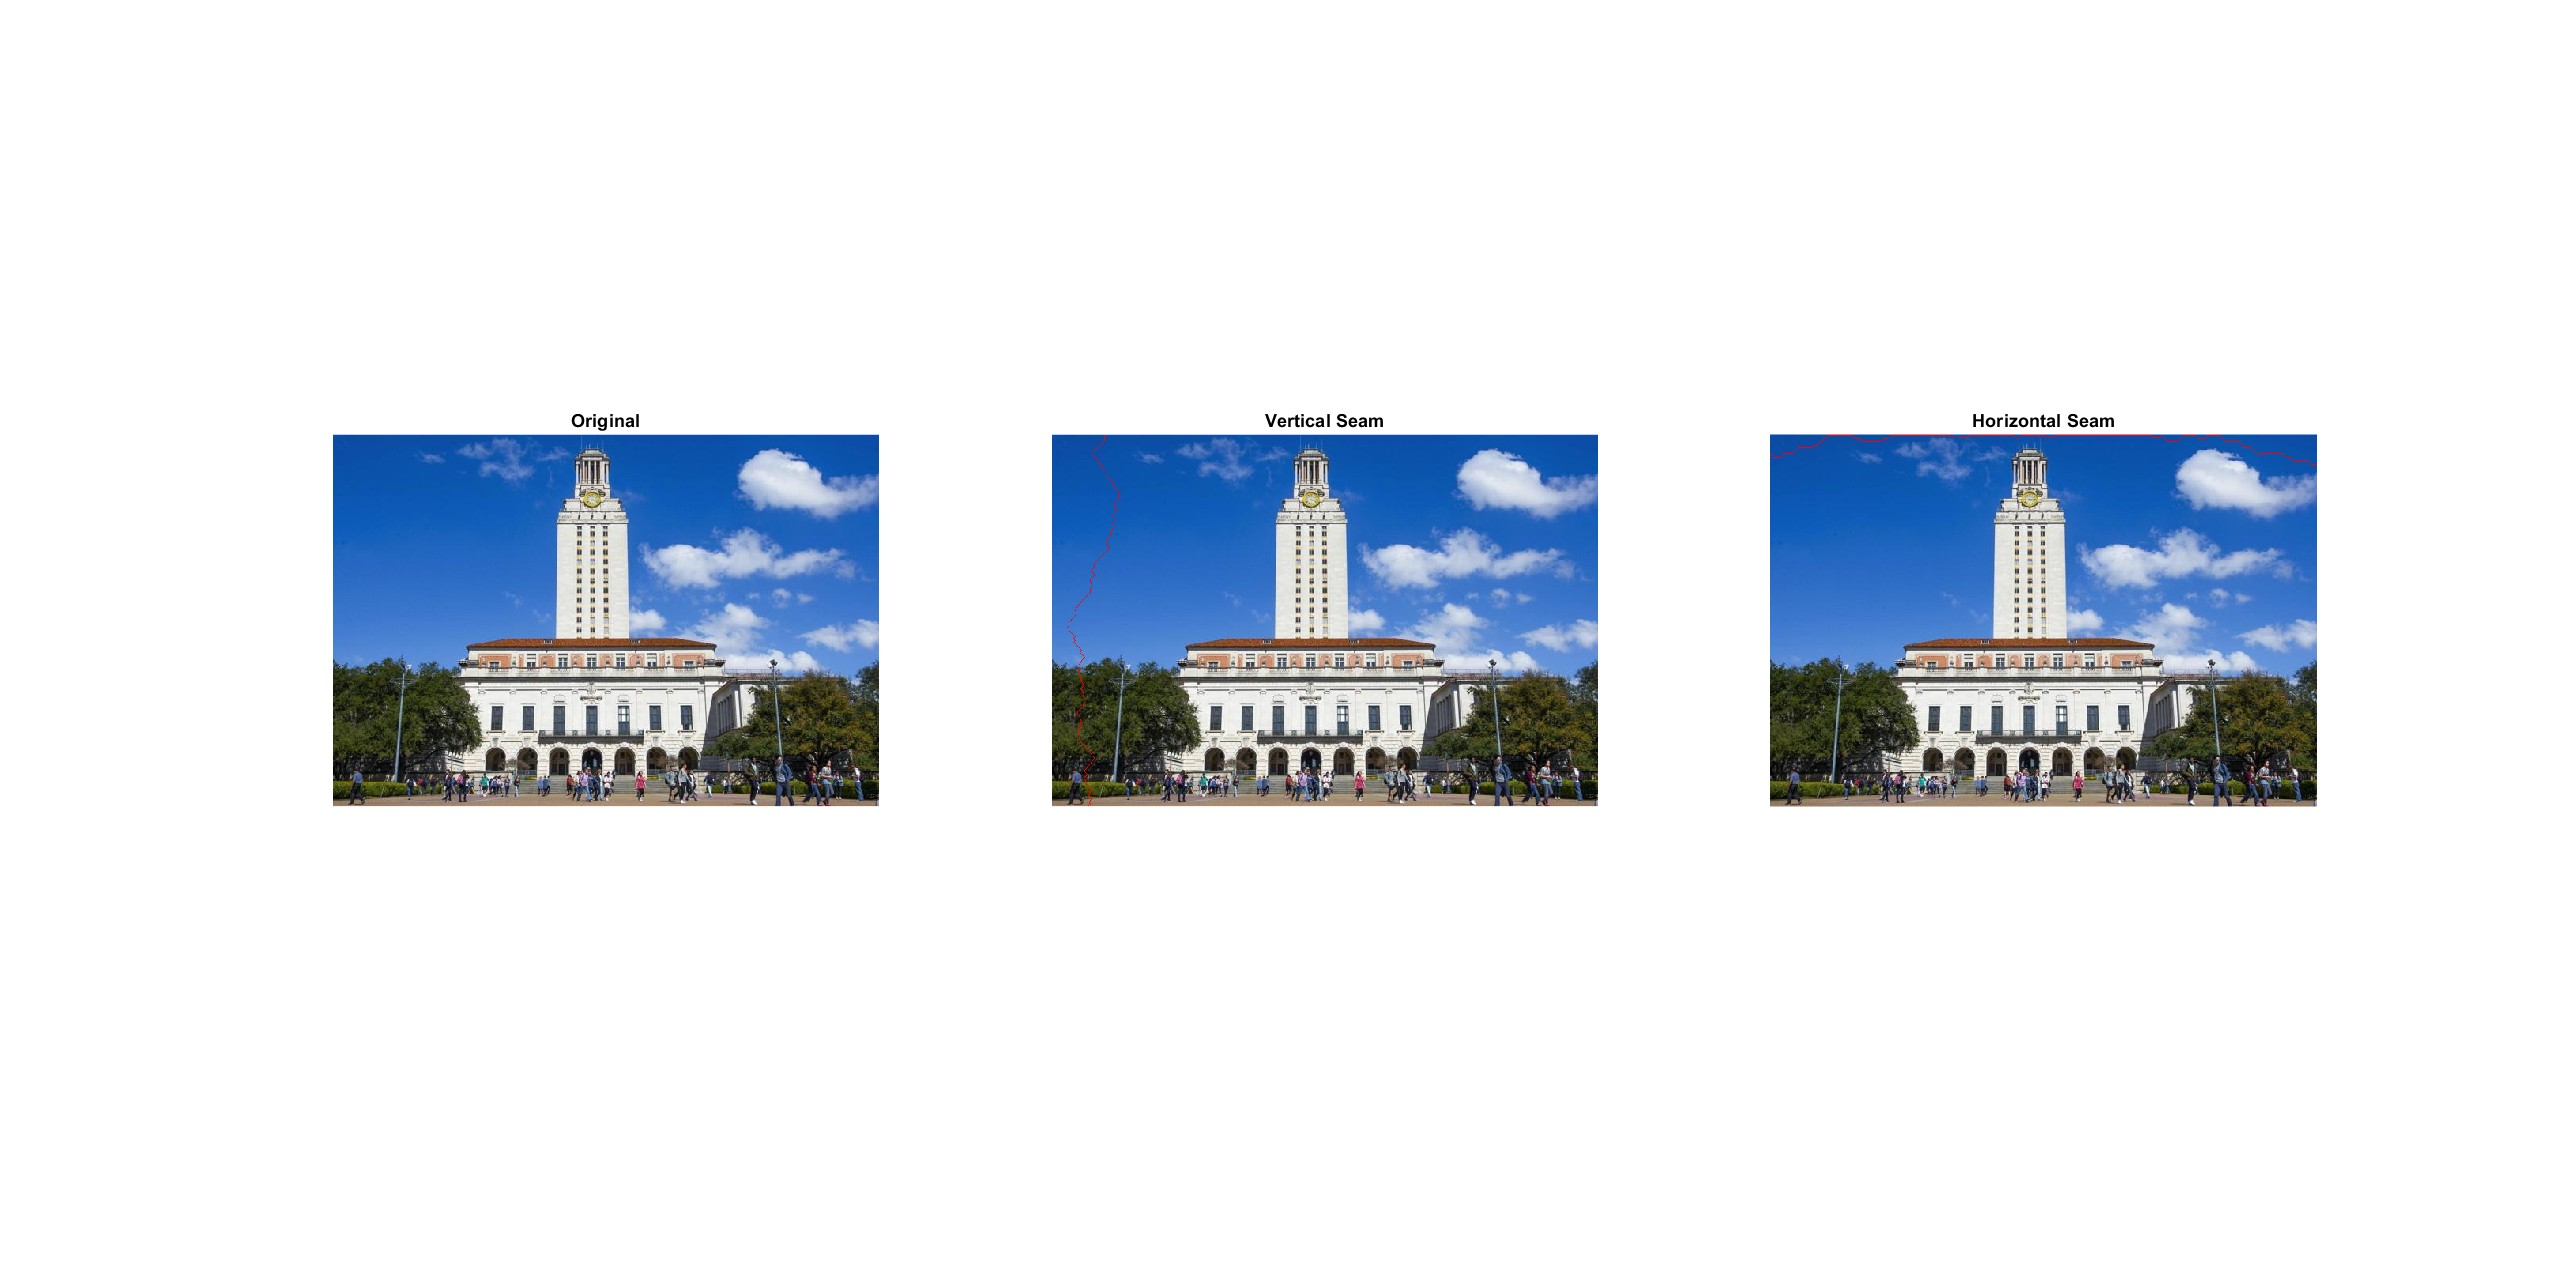
\includegraphics[width=\linewidth]{Part 2 Pictures/question3}\newline

    \textbf{Question 4:}\newline
    The results prove that blurring images first then calculating seams may
    produce different results then calculating seams then blurring the image.
    This is because the gradients of each pixel now are smaller since its
    value is closer to its neighbors.\newline
    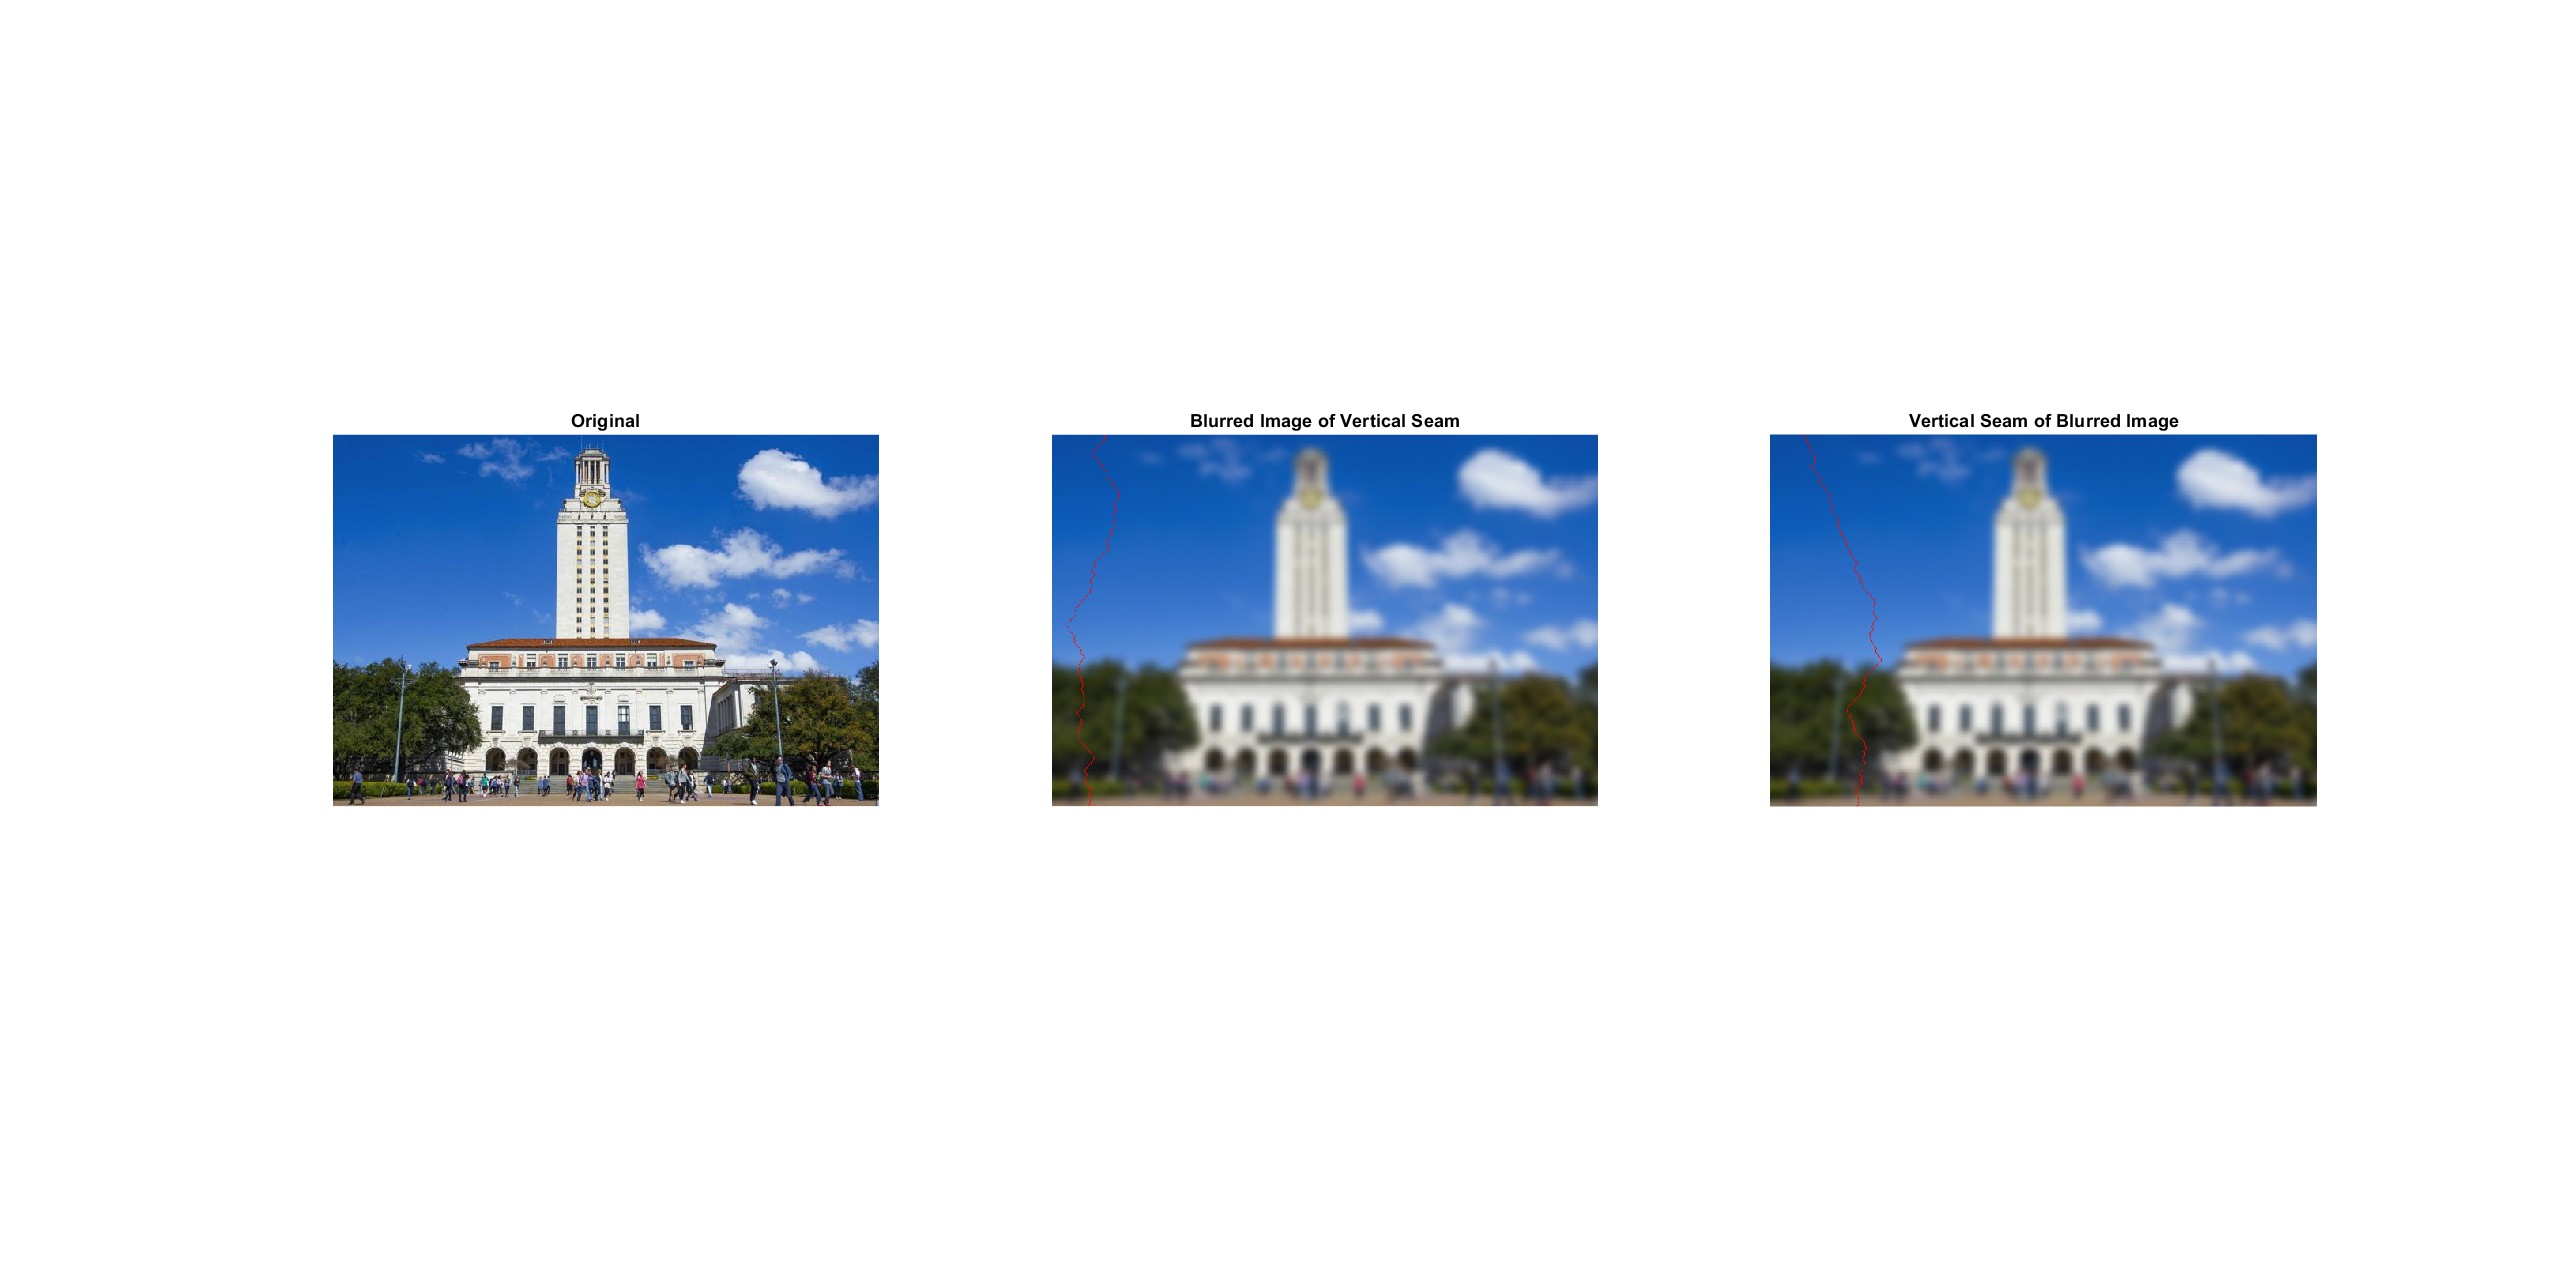
\includegraphics[width=\linewidth]{Part 2 Pictures/question4}\newline

    \textbf{Question 5:}\newline
    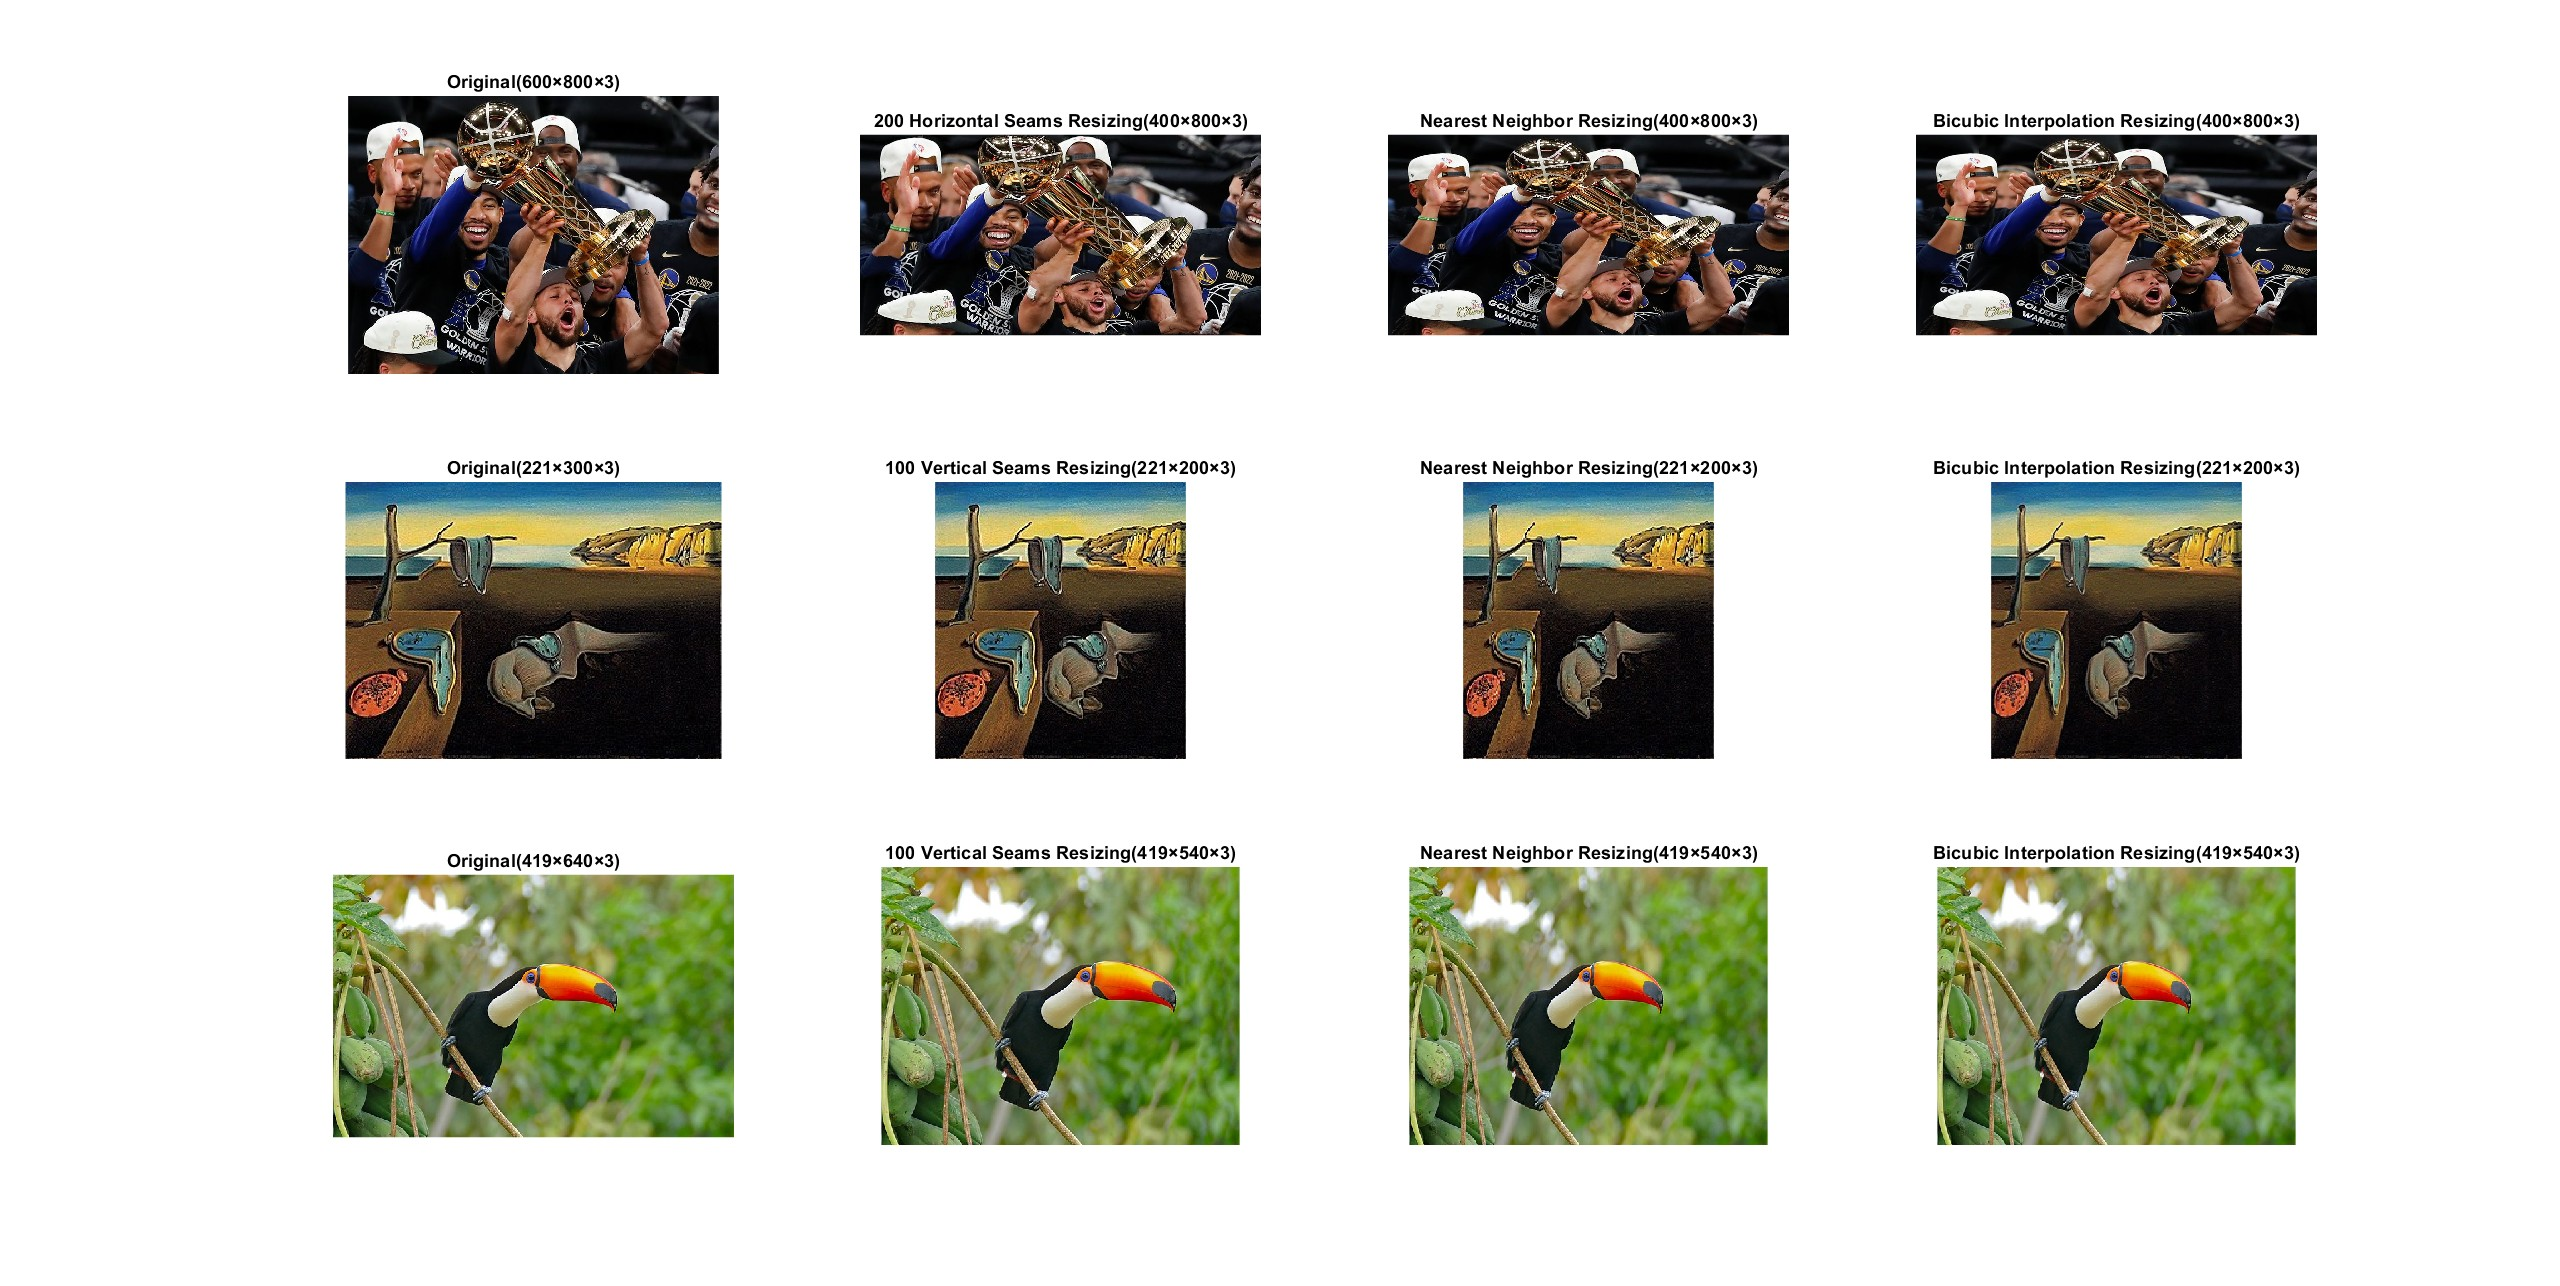
\includegraphics[width=\linewidth]{Part 2 Pictures/question5}\newline
\end{document}